\documentclass[border=15pt]{standalone}
\usepackage{tikz}
\usetikzlibrary{positioning, calc, arrows.meta, 3d, backgrounds}

% Color definitions matching PlotNeuralNet style
\definecolor{ConvColor}{HTML}{FFD54F}      % Yellow
\definecolor{PoolColor}{HTML}{FF8A65}      % Orange
\definecolor{HexColor}{HTML}{81C784}       % Green
\definecolor{FcColor}{HTML}{64B5F6}        % Blue
\definecolor{SoftmaxColor}{HTML}{BA68C8}   % Purple
\definecolor{InputColor}{HTML}{BDBDBD}     % Gray

\begin{document}
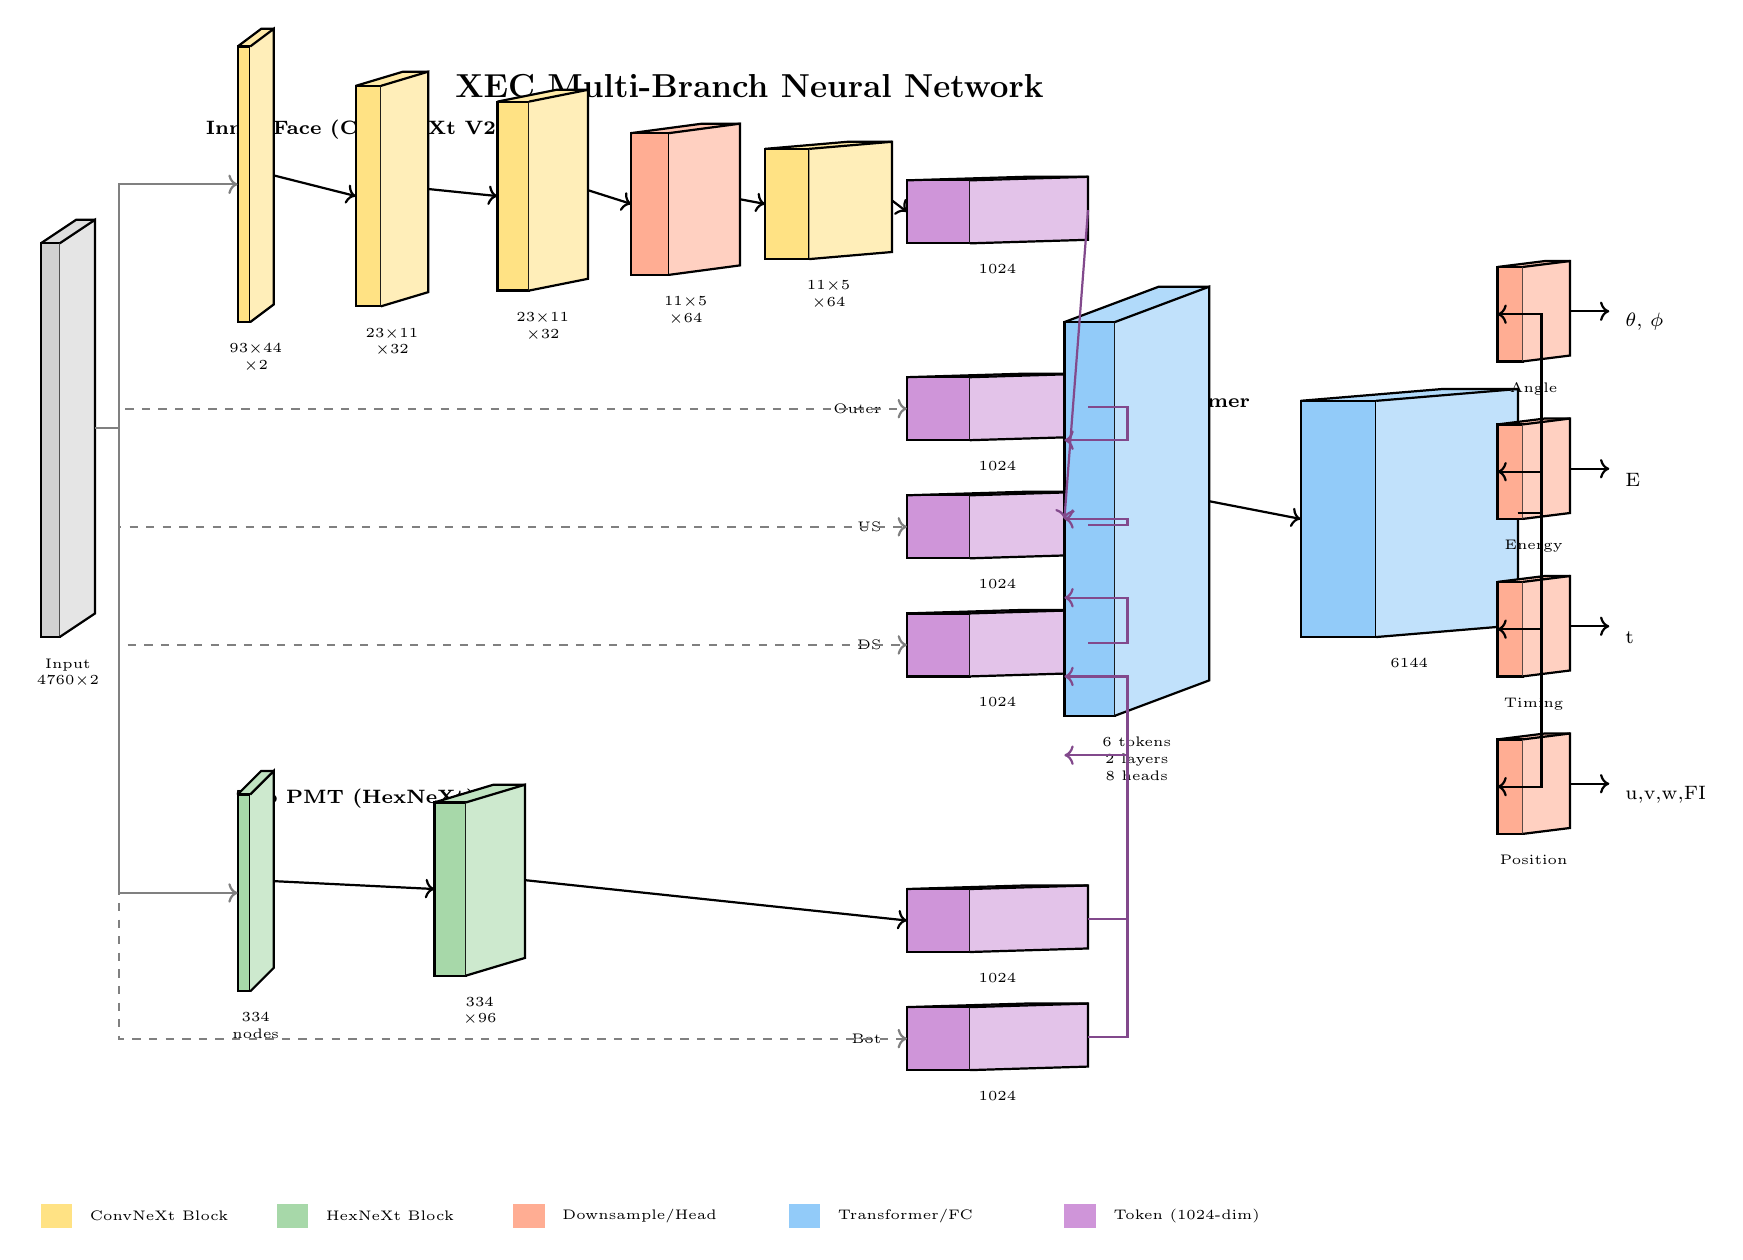
\begin{tikzpicture}[
    x=1cm, y=1cm,
    box/.style={draw, thick, minimum width=0.6cm},
]

% ============================================================
% MACRO: Draw a 3D feature map box
% #1=name, #2=x, #3=y, #4=height, #5=depth(visual), #6=width(channels), #7=color, #8=label
% ============================================================
\newcommand{\fmap}[8]{
    \begin{scope}[shift={(#2,#3)}]
        % Back face (for 3D effect)
        \fill[#7!30] (0.15*#6, 0.15*#5) rectangle (0.15*#6+0.08*#6, 0.15*#5+#4);
        % Top face
        \fill[#7!50] (0,#4) -- (0.15*#6, #4+0.15*#5) -- (0.15*#6+0.08*#6, #4+0.15*#5) -- (0.08*#6, #4) -- cycle;
        % Front face
        \fill[#7!70] (0,0) rectangle (0.08*#6, #4);
        \draw[thick] (0,0) rectangle (0.08*#6, #4);
        % Side face
        \fill[#7!40] (0.08*#6, 0) -- (0.08*#6+0.15*#6, 0.15*#5) -- (0.08*#6+0.15*#6, #4+0.15*#5) -- (0.08*#6, #4) -- cycle;
        \draw[thick] (0.08*#6, 0) -- (0.08*#6+0.15*#6, 0.15*#5) -- (0.08*#6+0.15*#6, #4+0.15*#5) -- (0.08*#6, #4);
        \draw[thick] (0,#4) -- (0.15*#6, #4+0.15*#5) -- (0.08*#6+0.15*#6, #4+0.15*#5);
        % Label
        \node[below, font=\tiny, align=center] at (0.04*#6+0.075*#6, -0.15) {#8};
        % Coordinate for connections
        \coordinate (#1-west) at (0, #4/2);
        \coordinate (#1-east) at (0.08*#6+0.15*#6, #4/2+0.075*#5);
        \coordinate (#1-center) at (0.04*#6+0.075*#6, #4/2+0.075*#5);
    \end{scope}
}

% ============================================================
% TITLE
% ============================================================
\node[font=\large\bfseries] at (9, 9) {XEC Multi-Branch Neural Network};

% ============================================================
% INPUT (4760 x 2)
% ============================================================
\fmap{input}{0}{2}{5}{2}{3}{InputColor}{Input\\4760$\times$2}

% ============================================================
% RECTANGULAR FACE PATH (ConvNeXt) - Inner Face Example
% ============================================================
\node[font=\scriptsize\bfseries, anchor=south] at (4, 8.2) {Inner Face (ConvNeXt V2)};

\fmap{inner-in}{2.5}{6}{3.5}{1.5}{2}{ConvColor}{93$\times$44\\$\times$2}
\fmap{inner-stem}{4}{6.2}{2.8}{1.2}{4}{ConvColor}{23$\times$11\\$\times$32}
\fmap{inner-b1}{5.8}{6.4}{2.4}{1}{5}{ConvColor}{23$\times$11\\$\times$32}
\fmap{inner-down}{7.5}{6.6}{1.8}{0.8}{6}{PoolColor}{11$\times$5\\$\times$64}
\fmap{inner-b2}{9.2}{6.8}{1.4}{0.6}{7}{ConvColor}{11$\times$5\\$\times$64}
\fmap{inner-tok}{11}{7}{0.8}{0.3}{10}{SoftmaxColor}{1024}

% Arrows for Inner path
\draw[->, thick, gray] (input-east) -- ++(0.3,0) |- (inner-in-west);
\draw[->, thick] (inner-in-east) -- (inner-stem-west);
\draw[->, thick] (inner-stem-east) -- (inner-b1-west);
\draw[->, thick] (inner-b1-east) -- (inner-down-west);
\draw[->, thick] (inner-down-east) -- (inner-b2-west);
\draw[->, thick] (inner-b2-east) -- (inner-tok-west);

% ============================================================
% OTHER RECTANGULAR FACES (simplified)
% ============================================================
\fmap{outer-tok}{11}{4.5}{0.8}{0.3}{10}{SoftmaxColor}{1024}
\fmap{us-tok}{11}{3}{0.8}{0.3}{10}{SoftmaxColor}{1024}
\fmap{ds-tok}{11}{1.5}{0.8}{0.3}{10}{SoftmaxColor}{1024}

\node[font=\tiny, anchor=east] at (10.8, 4.9) {Outer};
\node[font=\tiny, anchor=east] at (10.8, 3.4) {US};
\node[font=\tiny, anchor=east] at (10.8, 1.9) {DS};

% Dashed lines to show other paths
\draw[->, thick, gray, dashed] (input-east) -- ++(0.3,0) |- (2.5, 4.9) -- (outer-tok-west);
\draw[->, thick, gray, dashed] (input-east) -- ++(0.3,0) |- (2.5, 3.4) -- (us-tok-west);
\draw[->, thick, gray, dashed] (input-east) -- ++(0.3,0) |- (2.5, 1.9) -- (ds-tok-west);

% ============================================================
% HEXAGONAL FACE PATH (HexNeXt) - Top PMT Example
% ============================================================
\node[font=\scriptsize\bfseries, anchor=south] at (4, -0.3) {Top PMT (HexNeXt)};

\fmap{top-in}{2.5}{-2.5}{2.5}{2}{2}{HexColor}{334\\nodes}
\fmap{top-hex}{5}{-2.3}{2.2}{1.5}{5}{HexColor}{334\\$\times$96}
\fmap{top-tok}{11}{-2}{0.8}{0.3}{10}{SoftmaxColor}{1024}

\draw[->, thick, gray] (input-east) -- ++(0.3,0) |- (top-in-west);
\draw[->, thick] (top-in-east) -- (top-hex-west);
\draw[->, thick] (top-hex-east) -- (top-tok-west);

% Bottom PMT
\fmap{bot-tok}{11}{-3.5}{0.8}{0.3}{10}{SoftmaxColor}{1024}
\node[font=\tiny, anchor=east] at (10.8, -3.1) {Bot};
\draw[->, thick, gray, dashed] (input-east) -- ++(0.3,0) |- (2.5, -3.1) -- (bot-tok-west);

% ============================================================
% TRANSFORMER FUSION
% ============================================================
\node[font=\scriptsize\bfseries] at (14.5, 5) {Transformer};

\fmap{trans}{13}{1}{5}{3}{8}{FcColor}{6 tokens\\2 layers\\8 heads}

% Arrows to transformer
\draw[->, thick, SoftmaxColor!70!black] (inner-tok-east) -- (trans-west);
\draw[->, thick, SoftmaxColor!70!black] (outer-tok-east) -- ++(0.5,0) |- (13, 4.5);
\draw[->, thick, SoftmaxColor!70!black] (us-tok-east) -- ++(0.5,0) |- (13, 3.5);
\draw[->, thick, SoftmaxColor!70!black] (ds-tok-east) -- ++(0.5,0) |- (13, 2.5);
\draw[->, thick, SoftmaxColor!70!black] (top-tok-east) -- ++(0.5,0) |- (13, 1.5);
\draw[->, thick, SoftmaxColor!70!black] (bot-tok-east) -- ++(0.5,0) |- (13, 0.5);

% ============================================================
% TASK HEADS
% ============================================================
\fmap{concat}{16}{2}{3}{1}{12}{FcColor}{6144}

\draw[->, thick] (trans-east) -- (concat-west);

% Individual heads
\fmap{head-ang}{18.5}{5.5}{1.2}{0.5}{4}{PoolColor}{Angle}
\fmap{head-eng}{18.5}{3.5}{1.2}{0.5}{4}{PoolColor}{Energy}
\fmap{head-tim}{18.5}{1.5}{1.2}{0.5}{4}{PoolColor}{Timing}
\fmap{head-pos}{18.5}{-0.5}{1.2}{0.5}{4}{PoolColor}{Position}

\draw[->, thick] (concat-east) -- ++(0.3,0) |- (head-ang-west);
\draw[->, thick] (concat-east) -- ++(0.3,0) |- (head-eng-west);
\draw[->, thick] (concat-east) -- ++(0.3,0) |- (head-tim-west);
\draw[->, thick] (concat-east) -- ++(0.3,0) |- (head-pos-west);

% Output values
\node[font=\scriptsize, anchor=west] at (20, 6) {$\theta$, $\phi$};
\node[font=\scriptsize, anchor=west] at (20, 4) {E};
\node[font=\scriptsize, anchor=west] at (20, 2) {t};
\node[font=\scriptsize, anchor=west] at (20, 0) {u,v,w,FI};

\draw[->, thick] (head-ang-east) -- ++(0.5, 0);
\draw[->, thick] (head-eng-east) -- ++(0.5, 0);
\draw[->, thick] (head-tim-east) -- ++(0.5, 0);
\draw[->, thick] (head-pos-east) -- ++(0.5, 0);

% ============================================================
% LEGEND
% ============================================================
\begin{scope}[shift={(0,-5.5)}]
    \fill[ConvColor!70] (0,0) rectangle (0.4,0.3);
    \node[font=\tiny, anchor=west] at (0.5, 0.15) {ConvNeXt Block};

    \fill[HexColor!70] (3,0) rectangle (3.4,0.3);
    \node[font=\tiny, anchor=west] at (3.5, 0.15) {HexNeXt Block};

    \fill[PoolColor!70] (6,0) rectangle (6.4,0.3);
    \node[font=\tiny, anchor=west] at (6.5, 0.15) {Downsample/Head};

    \fill[FcColor!70] (9.5,0) rectangle (9.9,0.3);
    \node[font=\tiny, anchor=west] at (10, 0.15) {Transformer/FC};

    \fill[SoftmaxColor!70] (13,0) rectangle (13.4,0.3);
    \node[font=\tiny, anchor=west] at (13.5, 0.15) {Token (1024-dim)};
\end{scope}

\end{tikzpicture}
\end{document}
